\begin{tabular}{M{6.5cm}M{11cm}}
	\textbf{TRUNG TÂM MANABIE}& \textbf{ĐỀ ÔN TẬP KIỂM TRA CUỐI HỌC KÌ 1}\\
	\textbf{MÃ ĐỀ: 002}& \textbf{Bài thi môn: VẬT LÝ 12}\\
	\textit{(Đề trường THPT Lương Thế Vinh - Hà Nội năm học 2024 -2025)}& \textit{Thời gian làm bài: 50 phút, không kể thời gian phát đề}
	
	\noindent\rule{4cm}{0.8pt} \\
\end{tabular}
\setcounter{section}{0}
\section{Câu trắc nghiệm nhiều phương án lựa chọn}
\textit{Thí sinh trả lời từ câu 1 đến câu 18. Mỗi câu hỏi thí sinh chọn một phương án}
\setcounter{ex}{0}
\Opensolutionfile{ans}[ans/FINAL-SEM1-002-TN]
% ===================================================================
\begin{ex}
	Trong các chất sau, chất nào không phải là chất rắn kết tinh
	\choice
	{muối ăn}
	{thủy tinh}
	{kim cương}
	{thạch anh}
	\loigiai{}
\end{ex}
% ===================================================================
\begin{ex}
	Đặc điểm nào sau đây là đặc điểm của thể lỏng?
	\choice
	{Khoảng cách giữa các phân tử rất lớn so với kích thước của chúng}
	{Lực tương tác phân tử yếu hơn lực tương tác phân tử ở thể rắn}
	{Không có thể tích và hình dạng riêng xác định}
	{Các phân tử dao động xung quanh vị trí cân bằng xác định}
	\loigiai{}
\end{ex}
% ===================================================================
\begin{ex}
	Khi quan sát sự nóng chảy của nước đá tại nhiệt độ nóng chảy, trong suốt thời gian nóng chảy thì
	\choice
	{nhiệt độ của nước đá tăng}
	{nhiệt độ của nước đá giảm}
	{nhiệt độ của nước không thay đổi}
	{nhiệt độ của nước đá ban đầu tăng sau đó giảm}
	\loigiai{}
\end{ex}
% ===================================================================
\begin{ex}
	Sử dụng hai nhiệt kế rượu có độ chia từ $\SI{0}{\celsius}$ tới $\SI{100}{\celsius}$, hình vẽ nào trong hình bên dưới phù hợp với trường hợp nhiệt kế 1 được đặt vào một cốc đựng nước nóng còn nhiệt kế 2 được đặt vào một cốc nước lạnh?
	\begin{center}
		\includegraphics[scale=0.7]{../figs/FINAL-SEM1-002-1}
	\end{center}
	\choice
	{Hình B}
	{Hình C}
	{Hình A}
	{Hình D}
	\loigiai{}
\end{ex}
% ===================================================================
\begin{ex}
	\immini{Hiện tượng quả bóng bàn bị móp (nhưng chưa bị thủng) khi thả vào cốc nước nóng sẽ phồng trở lại là do nội năng của chất khí bên trong quả bóng}	
	{\vspace{-0.5cm}\includegraphics[scale=0.5]{../figs/FINAL-SEM1-002-2}}
	\choice
	{tăng lên}
	{giảm xuống}
	{không thay đổi}
	{giảm đi hai lần}
	\loigiai{}
\end{ex}
% ===================================================================
\begin{ex}
	Theo định luật I nhiệt động lực học $\Delta U=Q+A$. Biểu thức nào sau đây diễn tả quá trình biến thiên nội năng khi hệ nhận công và truyền nhiệt
	\choice
	{$\Delta U=Q+A$ với $Q>0$ và $A>0$}
	{$\Delta U=Q+A$ với $Q>0$ và $A<0$}
	{$\Delta U=Q+A$ với $Q<0$ và $A>0$}
	{$\Delta U=Q+A$ với $Q<0$ và $A<0$}
	\loigiai{}
\end{ex}
% ===================================================================
\begin{ex}
	Biết nhiệt nóng chảy riêng của nước đá là $\lambda=\SI{3.4E5}{\joule/\kilogram}$. Nhiệt lượng $Q$ cần cung cấp để làm nóng chảy $\SI{200}{\gram}$ nước đá ở $\SI{0}{\celsius}$ bằng
	\choice
	{$\SI{0.34E3}{\joule}$}
	{$\SI{340E5}{\joule}$}
	{$\SI{68E7}{\joule}$}
	{$\SI{68E3}{\joule}$}
	\loigiai{}
\end{ex}
% ===================================================================
\begin{ex}
	Biết nhiệt hóa hơi riêng của nước là $L=\SI{2.3E6}{\joule/\kilogram}$. Nhiệt lượng cần cung cấp để làm bay hơi hoàn toàn $\SI{300}{\gram}$ nước ở $\SI{100}{\celsius}$ là 
	\choice
	{$\SI{69E6}{\joule}$}
	{$\SI{6.9E5}{\joule}$}
	{$\SI{2.3E6}{\joule}$}
	{$\SI{0.23E4}{\joule}$}
	\loigiai{}
\end{ex}
% ===================================================================
\begin{ex}
\immini{Đồ thị biểu diễn hai đường đẳng nhiệt của cùng một lượng khí lí tưởng biểu diễn như hình vẽ. Mối quan hệ về nhiệt độ của hai đường đẳng nhiệt này là
	\choice
	{$T_2>T_1$}
	{$T_2=T_1$}
	{$T_2<T_1$}
	{$T_2\le T_1$}}
{\vspace{-0.5cm}	\includegraphics[scale=0.4]{../figs/FINAL-SEM1-002-3}}
	\loigiai{}
\end{ex}
% ===================================================================
\begin{ex}
	Một lượng khí có áp suất $\SI{750}{\milli\meter Hg}$, nhiệt độ $\SI{37}{\celsius}$ và thể tích $\SI{70}{\centi\meter^3}$. Thể tích khí ở điều kiện tiêu chuẩn (nhiệt độ $\SI{0}{\celsius}$ và áp suất $\SI{760}{\milli\meter Hg}$) có giá trị gần bằng
	\choice
	{$\SI{22.4}{\centi\meter^3}$}
	{$\SI{32.7}{\centi\meter^3}$}
	{$\SI{60.8}{\centi\meter^3}$}
	{$\SI{78}{\centi\meter^3}$}
	\loigiai{}
\end{ex}
% ===================================================================
\begin{ex}
Gọi $p$ là áp suất khối khí, $\mu$ là mật độ của phân tử khí, $m$ là khối lượng của phân tử khí, $\overline{v^2}$ là trung bình của bình phương tốc độ, $k$ là hằng số Boltzmann, $T$ là nhiệt độ tuyệt đối. Công thức nào sau đây mô tả đúng mối liên hệ giữa các đại lượng?	
	\choice
	{$p=\dfrac{2}{3}\mu m\overline{v^2}$}
	{$p=3\mu kT$}
	{$p=\mu kT$}
	{$p=\dfrac{3}{2}\mu m\overline{v^2}$}
	\loigiai{}
\end{ex}
% ===================================================================
\begin{ex}
Động năng trung bình của phân tử khí lí tưởng ở $\SI{37}{\celsius}$ có giá trị là	
	\choice
	{$\SI{5.21E-22}{\joule}$}
	{$\SI{6.42E-21}{\joule}$}
	{$\SI{6.24E23}{\joule}$}
	{$\SI{5.12E23}{\joule}$}
	\loigiai{}
\end{ex}
% ===================================================================
\begin{ex}
	Hình vẽ nào dưới đây biểu diễn đúng hướng của vector cảm ứng từ tại M gây ra bởi dòng điện trong dây dẫn thẳng dài vô hạn?
	\choice
	{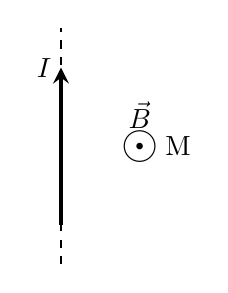
\begin{tikzpicture}
			\draw[dashed] (0,0)--(0,3);
			\draw[-stealth, line width=1.5pt] (0,0.5)--(0,2.5);
			\node at (1,1.5) {\LARGE $\odot$};
			\node[above] at (1,1.6) {$\vec{B}$};
			\node[left] at (0,2.5) {$I$};
			\node[right] at (1.2,1.5) {M};
	\end{tikzpicture}}
	{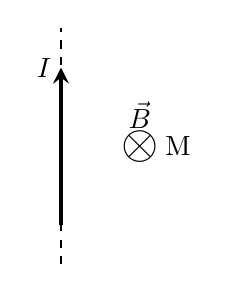
\begin{tikzpicture}
			\draw[dashed] (0,0)--(0,3);
			\draw[-stealth, line width=1.5pt] (0,0.5)--(0,2.5);
			\node at (1,1.5) {\LARGE $\otimes$};
			\node[above] at (1,1.6) {$\vec{B}$};
			\node[left] at (0,2.5) {$I$};
			\node[right] at (1.2,1.5) {M};
	\end{tikzpicture}}
	{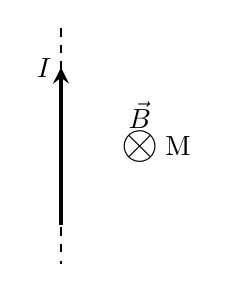
\begin{tikzpicture}
			\draw[dashed] (0,3)--(0,0);
			\draw[-stealth, line width=1.5pt] (0,0.5)--(0,2.5);
			\node at (1,1.5) {\LARGE $\otimes$};
			\node[above] at (1,1.6) {$\vec{B}$};
			\node[left] at (0,2.5) {$I$};
			\node[right] at (1.2,1.5) {M};
	\end{tikzpicture}}
	{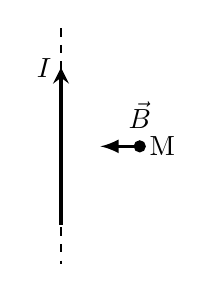
\begin{tikzpicture}
			\draw[dashed] (0,3)--(0,0);
			\draw[-stealth, line width=1.5pt] (0,0.5)--(0,2.5);
			\draw[-latex, line width=1.25pt] (1,1.5)--(0.5,1.5);
			\node[above] at (1,1.6) {$\vec{B}$};
			\node[left] at (0,2.5) {$I$};
			\filldraw (1,1.5) circle (2pt) node[right]{M};
	\end{tikzpicture}}
	\loigiai{}
\end{ex}
% ===================================================================
\begin{ex}
Hình nào sau đây biểu diễn không đúng vector lực từ tác dụng đoạn dây dẫn mang dòng điện đặt trong từ trường đều	
\begin{center}
	\begin{tabular}{M{4cm}M{4cm}M{4cm}M{4cm}}
		\begin{tikzpicture}
			\coordinate(A) at(0.2,0.2);
			\coordinate(B) at($(A)+(30:2.5)$);
			\foreach \x in {0,2}{
				\foreach \y in {0,2}{
					\node at (\x,\y) {\LARGE$\otimes$};
				}
			};
			\draw[-stealth, line width=1.5pt, blue] ($(A)!0.5!(B)$)--+(120:1.5);
			\draw[line width=4pt, gray,decoration={markings, mark=at position 0.5 with {\arrow{stealth}}},
			postaction={decorate}] (A)--(B);
			\node[below] at ($(A)!0.5!(B)$) {$I$};
			\node[right, blue] at ($(A)!0.5!(B)+(120:1.5)$) {$\vec{F}$};
			\node[right] at (2.1,2) {$\vec{B}$};
		\end{tikzpicture}
		&
		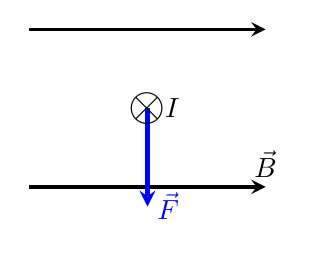
\begin{tikzpicture}
			\draw[-stealth, line width=1.25pt] (0,0)--(3,0);
			\draw[-stealth, line width=1.25pt] (0,2)--(3,2);
			\draw[-stealth, blue, line width=1.5pt] (1.5,1)--(1.5,-0.25);
			\node at(1.5,1) {\LARGE$\otimes$};
			\node[right] at(1.6,1) {$I$};
			\node[right, blue] at(1.5,-0.25) {$\vec{F}$};
			\node[above] at(3,0) {$\vec{B}$};
		\end{tikzpicture}
		&
		\begin{tikzpicture}
			\draw[-stealth, line width=1.25pt] (0,0)--(3,0);
			\draw[-stealth, line width=1.25pt] (0,2)--(3,2);
			\draw[-stealth, blue, line width=1.5pt] (1.5,1)--(1.5,2.25);
			\draw[line width=4pt, gray,decoration={markings, mark=at position 0.5 with {\arrow{stealth}}},
			postaction={decorate}] (0.5,1)--(2.5,1);
			\node[below] at(1.6,1) {$I$};
			\node[right, blue] at(1.5,2.25) {$\vec{F}$};
			\node[above] at(3,0) {$\vec{B}$};
		\end{tikzpicture}
		&
		\begin{tikzpicture}
			\coordinate(A) at (0.2,-0.2);
			\coordinate(B) at ($(A)+(-30:2.5)$);
			\draw[-stealth, line width=1.25pt] (0,0)--(0,-2);
			\draw[-stealth, line width=1.25pt] (2.5,0)--(2.5,-2);
			\draw[line width=4pt, gray,decoration={markings, mark=at position 0.5 with {\arrow{stealth}}},
			postaction={decorate}] (A)--(B);
			\node[above] at($(A)!0.5!(B)+(0,0.1)$) {$I$};
			\node[below, blue] at($(A)!0.5!(B)-(0,0.2)$) {$\vec{F}$};
			\node[above] at(3,0) {$\vec{B}$};
			\node[fill=none] at ($(A)!0.5!(B)$) {\LARGE$\otimes$};
		\end{tikzpicture}\\
		\textbf{Hình 1} & \textbf{Hình 2} & \textbf{Hình 3} & \textbf{Hình 4}
	\end{tabular}
\end{center}
	\choice
	{Hình 1}
	{Hình 2}
	{Hình 3}
	{Hình 4}
	\loigiai{}
\end{ex}
% ===================================================================
\begin{ex}
Một quả bóng có dung tích $\SI{2.5}{\liter}$. Người ta bơm không khí ở áp suất $\SI{E5}{\pascal}$ vào bóng. Mỗi lần bơm được $\SI{150}{\centi\meter^3}$ không khí. Tính áp suất của không khí trong quả bóng sau 50 lần bơm. Coi quả bóng trước khi bơm không có không khí và nhiệt độ trong quả bóng không thay đổi.
	\choice
	{$\SI{25E5}{\pascal}$}
	{$\SI{2.5E5}{\pascal}$}
	{$\SI{0.25E5}{\pascal}$}
	{$\SI{3E5}{\pascal}$}
	\loigiai{}
\end{ex}
% ===================================================================
\begin{ex}
	Ba chất lỏng không tác dụng hóa học với nhau và được trộn lẫn vào nhau trong một nhiệt lượng kế; chúng có khối lượng lần lượt là $m_1=\SI{1}{\kilogram}$, $m_2=\SI{10}{\kilogram}$, $m_3=\SI{5}{\kilogram}$ có nhiệt dung riêng lần lượt là $c_1=\SI{2000}{\kilogram\cdot\kelvin}$; $c_2=\SI{4000}{\joule/\kilogram\cdot\kelvin}$; $c_3=\SI{2500}{\joule/\kilogram\cdot\kelvin}$ và có nhiệt độ là $t_1=\SI{6}{\celsius}$; $t_2=\SI{20}{\celsius}$; $t_3=\SI{-60}{\celsius}$. Bỏ qua sự trao đổi nhiệt với nhiệt lượng kế và với môi trường. Nhiệt độ của hỗn hợp khi xảy ra cân bằng nhiệt xấp xỉ
	\choice
	{$\SI{-2.5}{\celsius}$}
	{$\SI{-1.9}{\celsius}$}
	{$\SI{1.1}{\celsius}$}
	{$\SI{3.5}{\celsius}$}
	\loigiai{}
\end{ex}
% ===================================================================
\begin{ex}
	Khí helium có khối lượng mol phân tử là $\SI{4}{\gram/\mole}$. Coi các phân tử khí là giống nhau. Trung bình của bình phương tốc độ trong chuyển động nhiệt của phân tử khí helium ở nhiệt độ $\SI{320}{\kelvin}$ là
	\choice
	{$\SI{1.995E6}{\meter^2/\second^2}$}
	{$\SI{2.01E6}{\meter^2/\second^2}$}
	{$\SI{2010}{\meter^2/\second^2}$}
	{$\SI{2020}{\meter^2/\second^2}$}
	\loigiai{}
\end{ex}
% ===================================================================
\begin{ex}
	Treo đoạn dây dẫn có chiều dài $\ell=\SI{10}{\centi\meter}$, khối lượng $m=\SI{5}{\gram}$ bằng hai dây mảnh, nhẹ sao cho dây dẫn nằm ngang. Biết cảm ứng từ của từ trường hướng thẳng đứng xuống dưới, có độ lớn $B=\SI{0.5}{\tesla}$ và dòng điện đi qua dây dẫn là $I=\SI{1}{\ampere}$. Lấy $g=\SI{10}{\meter/\second^2}$ thì góc lệch của dây treo so với phương thẳng đứng là
	\choice
	{$\SI{30}{\degree}$}
	{$\SI{45}{\degree}$}
	{$\SI{60}{\degree}$}
	{$\SI{90}{\degree}$}
	\loigiai{}
\end{ex}
\Closesolutionfile{ans}
\section{Câu trắc nghiệm đúng/sai} 
\textit{Thí sinh trả lời từ câu 1 đến câu 4. Trong mỗi ý \textbf{a)}, \textbf{b)}, \textbf{c)}, \textbf{d)} ở mỗi câu, thí sinh chọn đúng hoặc sai}
\setcounter{ex}{0}
\Opensolutionfile{ans}[ans/FINAL-SEM1-002-TF]
% ===================================================================
\begin{ex}
	Cho đồ thị biểu diễn sự thay đổi nhiệt độ của nước theo thời gian đun như hình bên. Biết nhiệt độ nóng chảy của nước đá là $\SI{0}{\celsius}$, nhiệt độ sôi của nước là $\SI{100}{\celsius}$.
\begin{center}
		\begin{tikzpicture}  
		\begin{axis}[  ultra thick,
			xmin=0,  
			xmax=34,  
			xtick={0,5,...,35},
			ytick={-10,0,...,120},
			minor x tick num=1,
			minor y tick num=0,
			ymin=-10,  
			ymax=110, 
			samples=300,
			yticklabels=\empty,
			axis lines=center, 
			grid style={step=1, line width=0.8pt,gray!60!white},
			grid=both, %giới hạn ô lưới
			major grid style={line width=0.8pt,gray!60!white},
			xlabel=$\xsi{t}{\left(\minute\right)}$, 		
			ylabel=$\text{Nhiệt độ}\ \left(\si{\celsius}\right)$,
			every axis y label/.style={at=(current axis.above origin),anchor=south},  
			every axis x label/.style={at=(current axis.right of origin),anchor=south},  ]
			\coordinate (A) at (axis cs: 0,-10);
			\coordinate (B) at (axis cs: 5,0);
			\coordinate (C) at (axis cs: 10,0);
			\coordinate (D) at (axis cs: 25,100);
			\coordinate (E) at (axis cs: 30,100);
			\draw[line width=1.5pt,blue] plot coordinates {(A) (B) (C) (D) (E)};
			\coordinate (O) at (axis cs: 0,0);
			\coordinate (t1) at (axis cs: 0,-10);
			\coordinate (t2) at (axis cs: 0,100);
		\end{axis}  
		\node[left] at (O) {0};
		\node[left] at (t1) {$-10$};
		\node[left] at (t2) {$100$};
	\end{tikzpicture}
\end{center}
	\choiceTF[t]
	{}
	{}
	{}
	{}
	\loigiai{}
\end{ex}
\Closesolutionfile{ans}
\section{Câu trắc nghiệm trả lời ngắn} \textit{Thí sinh trả lời từ câu 1 đến câu 6}
\setcounter{ex}{0}
\Opensolutionfile{ans}[ans/FINAL-SEM1-002-TL]
% ===============================================================
\begin{ex}
	
	\shortans[oly]{ }
	\loigiai{
		
	}
\end{ex}


\Closesolutionfile{ans}
